\section{\textbf{Nos preguntamos:} ¿En qué negocio estamos?}
\begin{itemize}
    \item La empresa está a veces alineada con el target y alineada con el producto, cuando esto no está alineado surgen cosas conflictivas.
    \item \textbf{Nos preguntamos:} ¿En qué negocio estoy en lugar de qué negocio \textbf{creo} que estoy?
    \item \begin{figure}[htbp]
        \centering
        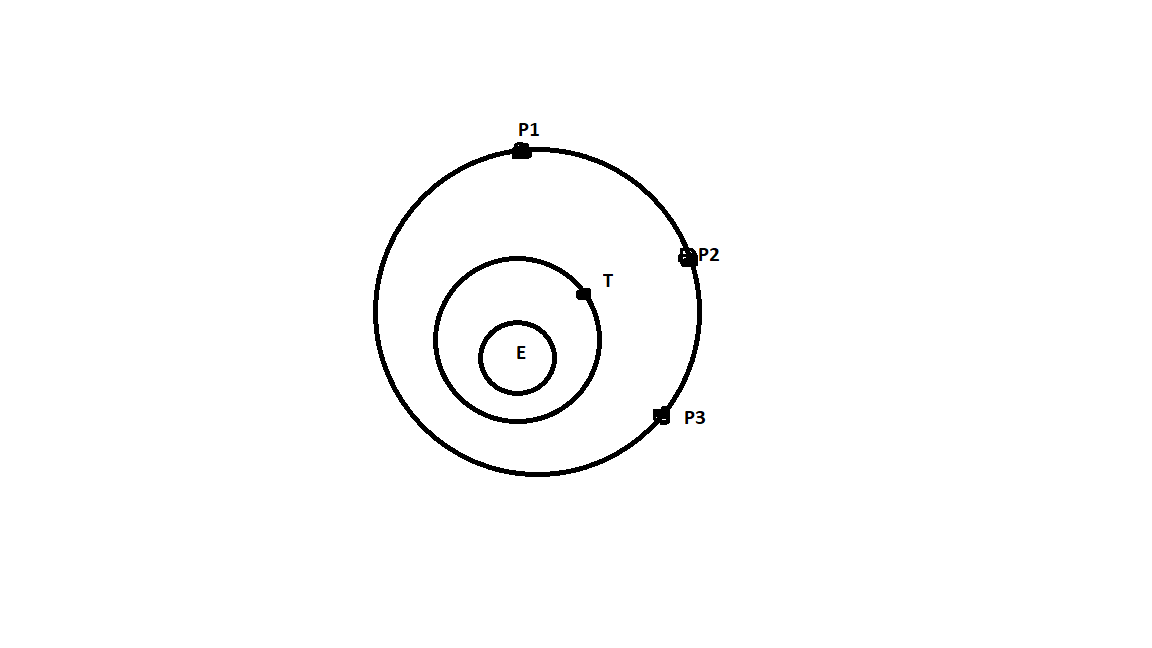
\includegraphics[width=8cm]{./../__Imagenes__/2020-01-21-MARKETING.png}
        \caption{E $\rightarrow$ Empresa; P $\rightarrow$ Productos; T $\rightarrow$ Target}
        \label{}
    \end{figure}
\end{itemize}

%%%%%%%%%%%%%%%%%%%%%%%%%%%%%%%%%%%%%%%%%%%%%%%%%%%%%%%%%%%%%%%%%%%%%%%%%%%%%%%%%%%%%%%%%%%%%%%%

\subsection{Ejemplos}
\begin{itemize}
    \item Starbucks está en el negocio de la leche.
    \item Membresía de gimnasio.
    \item 
\end{itemize}
